\section{Gestión del Alcance}\label{sec:gestionDelAlcance}

La Gestión del Alcance del Proyecto incluye los procesos necesarios para garantizar que el proyecto incluya todo el 
trabajo requerido y únicamente el trabajo para completar el proyecto con éxito. Gestionar el alcance del proyecto se 
enfoca primordialmente en definir y controlar qué se incluye y qué no se incluye en el proyecto.

\subsection{Definir el Alcance}

Es el proceso de desarrollar una descripción detallada del proyecto y del producto. El alcance del proyecto está limitado 
por el tiempo, ya que se debe cumplir con fechas establecidas por la universidad. Por lo tanto, es importante definir las 
funcionalidades del proyecto de manera eficiente para poder cumplir con el alcance dentro del tiempo establecido.

Para definir el alcance se utilizará la Agile Planning Onion que define las siguientes etapas:
[cita: https://www.productplan.com/blog/agile-planning-onion/]

\begin{itemize}
    \item \textbf{Visión:} Define los objetivos generales y el valor que el producto aportará.
    \item \textbf{Hoja de Ruta (Roadmap):} Describe planes de alto nivel para alcanzar la visión, incluyendo metas a largo plazo.
    \item \textbf{Planificación de Releases:} Detalla las características específicas que se entregarán en cada versión del producto.
    \item \textbf{Planificación de Iteraciones:} Planifica las tareas para las próximas semanas, definiendo acciones concretas.
    \item \textbf{Planificación Diaria:} Reuniones diarias para evaluar el progreso y planificar el trabajo del día.
\end{itemize}

Para este proyecto haremos una adaptación eliminando la Planificación diaria.

\subsubsection{Visión}

\begin{figure}[H]
    \centering
    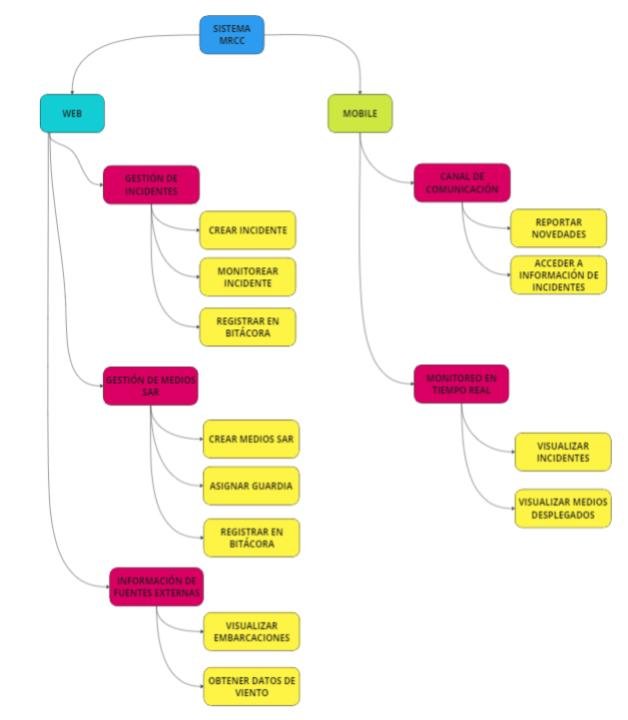
\includegraphics[width=0.8\textwidth]{../imagenes/secciones/6-Gestion-del-proyecto/vision.jpg}
    \caption{Visión del proyecto}
    \label{fig:vision}
\end{figure}

\subsubsection{Roadmap}

\begin{figure}[H]
    \centering
    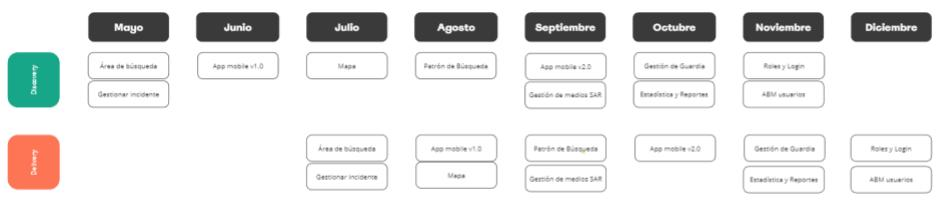
\includegraphics[width=0.8\textwidth]{../imagenes/secciones/6-Gestion-del-proyecto/roadmap.jpg}
    \caption{Roadmap del proyecto}
    \label{fig:roadmap}
\end{figure}

\subsubsection{Planificación de Releases}

\begin{figure}[H]
    \centering
    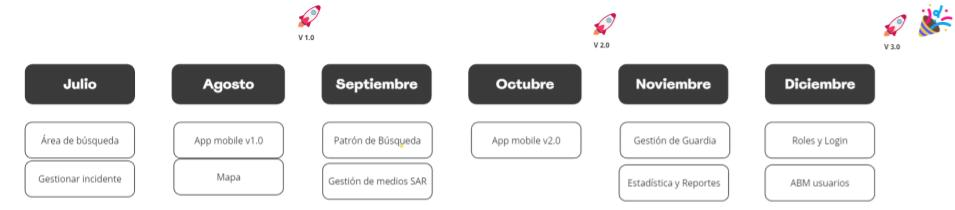
\includegraphics[width=0.8\textwidth]{../imagenes/secciones/6-Gestion-del-proyecto/releases.jpg}
    \caption{Planificación de Releases}
    \label{fig:releases}
\end{figure}

\subsubsection{Planificación de Iteraciones}

En la etapa de delivery desarrollaremos las historias de usuario obtenidas durante la el track de discovery. 
Se planifica realizar 12 sprints a lo largo de 5 releases entre julio y diciembre.


\subsection{Story Mapping}

El Story Mapping es una técnica ágil que permite visualizar y organizar el trabajo necesario para desarrollar un 
producto, dividiendo el trabajo en historias de usuario y organizándose en un flujo de actividades de usuario. 
Esto es especialmente útil para nuestro proyecto de sistema de gestión de incidentes de búsqueda y rescate, ya que 
nos permitirá estructurar y priorizar el desarrollo de funcionalidades de manera efectiva.

\subsubsection{ Definir el Objetivo del Proyecto}
Desarrollar un sistema centralizado y automatizado para la gestión de incidentes de búsqueda y rescate en el mar, 
mejorando la eficiencia y efectividad de las operaciones del MRCC Uruguay.

\subsubsection{Identificar a los Actores Clave}
Operadores del MRCC: Responsables de gestionar incidentes de búsqueda y rescate.
Personal de la Armada: Involucrados en las operaciones de rescate.
Stakeholders Clave: Contralmirante Vizcay y Capitán Javier Calvo.

\subsubsection{Mapeo del Recorrido del Usuario}
Visualizar todas las etapas que un operador del MRCC atraviesa desde el momento en que recibe un incidente hasta su 
resolución.

\subsubsubsection{Etapas del Recorrido del Usuario}

\begin{itemize}
    \item Recepción del Incidente: Recibir la notificación de un incidente.
    \item Análisis de Información: Recolectar y analizar la información del incidente.
    \item Cálculo del Área de Búsqueda: Realizar cálculos para determinar la posible ubicación de la embarcación en peligro.
    \item Despliegue de Recursos: Enviar equipos de rescate y coordinar las operaciones.
    \item Monitoreo y Comunicación: Monitorear el progreso y mantener la comunicación con los equipos de rescate.
    \item Resolución del Incidente: Concluir el rescate y proporcionar asistencia necesaria.
    \item Documentación y Reportes: Documentar el incidente y generar reportes detallados.
\end{itemize}


\subsubsection{Identificar y Crear Épicas y Historias de Usuario}

Dividir el recorrido del usuario en historias de usuario que describen las necesidades y funcionalidades específicas.

\subsubsubsection{Épica 1: Área de búsqueda}
\begin{itemize}
    \item \textbf{Historia 1.1:} Como operador del MRCC, quiero calcular la ubicación más probable de un objeto buscado (DATUM) para planificar la operación de rescate.
\end{itemize}

\subsubsubsection{Épica 2: Gestionar Incidente}

\begin{itemize}
    \item \textbf{Historia 2.1:} Como operador del MRCC, quiero registrar incidentes en una interfaz centralizada para mantener 
    toda la información relevante organizada.
    \item \textbf{Historia 2.2:} Como operador del MRCC, quiero buscar incidentes pasados para poder revisar los hechos ocurridos.
    \item \textbf{Historia 2.3:} Como operador del MRCC, quiero poder asignar medios SAR a un incidente para que los mismos reciban 
    toda la información relativa al incidente.
    \item \textbf{Historia 2.4:} Como operador del MRCC, quiero mantener una bitácora detallada de cada incidente para documentar 
    todas las acciones y decisiones tomadas durante el rescate.
    \item \textbf{Historia 2.5:} Como operador del MRCC, quiero poder imprimir/exportar como pdf la bitácora de un incidente para 
    poder firmar el relevo de guardia.
\end{itemize}

\subsubsubsection{Épica 3: Mapa }

\begin{itemize}
    \item \textbf{Historia 3.1:} Como operador del MRCC, quiero visualizar en el mapa las embarcaciones registradas para coordinar 
    mejor las operaciones de rescate.
    \item \textbf{Historia 3.2:} Como operador del MRCC, quiero obtener información detallada de las embarcaciones cercanas al incidente 
    para solicitar su asistencia si es necesario.
    \item \textbf{Historia 3.3:} Como operador del MRCC, quiero poder agregar la última posición conocida del objeto a buscar para poder 
    hacer la planificación de búsqueda.
    \item \textbf{Historia 3.4:} Como operador del MRCC, quiero visualizar el área de búsqueda  y los medios SAR asignados al incidente 
    en el mapa para poder monitorear la evolución del incidente.
    \item \textbf{Historia 3.5:} Como operador del MRCC, quiero poder generar capas de áreas de búsqueda para poder visualizarlas en el mapa.
    \item \textbf{Historia 3.6:} Como operador del MRCC, quiero poder mostrar el patrón de búsqueda en el mapa para poder coordinar las 
    operaciones de búsqueda.
\end{itemize}

\subsubsubsection{Épica 4: Patrón de Búsqueda }

\begin{itemize}
    \item \textbf{Historia 4.1:} Como operador del MRCC, quiero seleccionar y configurar el patrón de búsqueda para planificar la 
    ejecución del incidente.
    \item \textbf{Historia 4.2:} Como operador del MRCC, exportar el patrón de búsqueda para que pueda ser importado en una carta 
    náutica electrónica para reducir errores humanos y agilizar la operación de búsqueda.
\end{itemize}

\subsubsubsection{Épica 5: Gestión de Medios SAR }

\begin{itemize}
    \item \textbf{Historia 5.1:} Como administrador del sistema, quiero gestionar la información de los medios disponibles para mantener 
    la base de datos actualizada.
    \item \textbf{Historia 5.2:} Como operador del MRCC quiero actualizar la situación diaria de los medios SAR para saber si están 
    disponibles para posibles operaciones de rescate.
\end{itemize}

\subsubsubsection{Épica 6: Gestión de Guardia }

\begin{itemize}
    \item \textbf{Historia 6.1:} Como operador del MRCC, quiero poder registrar el relevo de guardia para mantener un registro de las 
    novedades y decisiones tomadas.
    \item \textbf{Historia 6.2:} Como operador del MRCC, quiero poder generar informes de novedades diarias para mantener a todos los 
    involucrados informados.
    \item \textbf{Historia 6.3:} Como operador del MRCC, quiero distribuir automáticamente los informes de novedades a los stakeholders 
    relevantes para asegurar una comunicación efectiva.
\end{itemize}

\subsubsubsection{Épica 7: Estadística y Reportes }

\begin{itemize}
    \item \textbf{Historia 7.1:} Como operador del MRCC, quiero generar estadísticas detalladas de los incidentes y las operaciones
    de rescate para analizar el desempeño y mejorar continuamente.
    \item \textbf{Historia 7.2:} Como administrador del sistema, quiero exportar reportes en diferentes formatos para facilitar la 
    presentación y el análisis de datos.
\end{itemize}

\subsubsubsection{Épica 8: Roles y Login }

\begin{itemize}
    \item \textbf{Historia 8.1:} Como administrador del sistema, quiero definir y gestionar roles y permisos de usuario para asegurar 
    que cada miembro del equipo tenga acceso adecuado a las funcionalidades del sistema.
    \item \textbf{Historia 8.2:} Como operador del MRCC, quiero ver y realizar solo las acciones permitidas según mi rol para evitar 
    errores y mejorar la seguridad del sistema.
\end{itemize}

\subsubsubsection{Épica 9: ABM Usuarios}

\begin{itemize}
    \item \textbf{Historia 9.1:} Como administrador del sistema, quiero gestionar la información de los usuarios, incluyendo su registro, 
    actualización y eliminación, para mantener la base de datos de usuarios actualizada.
    \item \textbf{Historia 9.2:} Como administrador del sistema, quiero asignar roles y permisos a los usuarios para controlar el acceso 
    a las diferentes funcionalidades del sistema.
\end{itemize}
